\documentclass[twoside]{book}

% Packages required by doxygen
\usepackage{fixltx2e}
\usepackage{calc}
\usepackage{doxygen}
\usepackage[export]{adjustbox} % also loads graphicx
\usepackage{graphicx}
\usepackage[utf8]{inputenc}
\usepackage{makeidx}
\usepackage{multicol}
\usepackage{multirow}
\PassOptionsToPackage{warn}{textcomp}
\usepackage{textcomp}
\usepackage[nointegrals]{wasysym}
\usepackage[table]{xcolor}

% Font selection
\usepackage[T1]{fontenc}
\usepackage[scaled=.90]{helvet}
\usepackage{courier}
\usepackage{amssymb}
\usepackage{sectsty}
\renewcommand{\familydefault}{\sfdefault}
\allsectionsfont{%
  \fontseries{bc}\selectfont%
  \color{darkgray}%
}
\renewcommand{\DoxyLabelFont}{%
  \fontseries{bc}\selectfont%
  \color{darkgray}%
}
\newcommand{\+}{\discretionary{\mbox{\scriptsize$\hookleftarrow$}}{}{}}

% Page & text layout
\usepackage{geometry}
\geometry{%
  a4paper,%
  top=2.5cm,%
  bottom=2.5cm,%
  left=2.5cm,%
  right=2.5cm%
}
\tolerance=750
\hfuzz=15pt
\hbadness=750
\setlength{\emergencystretch}{15pt}
\setlength{\parindent}{0cm}
\setlength{\parskip}{3ex plus 2ex minus 2ex}
\makeatletter
\renewcommand{\paragraph}{%
  \@startsection{paragraph}{4}{0ex}{-1.0ex}{1.0ex}{%
    \normalfont\normalsize\bfseries\SS@parafont%
  }%
}
\renewcommand{\subparagraph}{%
  \@startsection{subparagraph}{5}{0ex}{-1.0ex}{1.0ex}{%
    \normalfont\normalsize\bfseries\SS@subparafont%
  }%
}
\makeatother

% Headers & footers
\usepackage{fancyhdr}
\pagestyle{fancyplain}
\fancyhead[LE]{\fancyplain{}{\bfseries\thepage}}
\fancyhead[CE]{\fancyplain{}{}}
\fancyhead[RE]{\fancyplain{}{\bfseries\leftmark}}
\fancyhead[LO]{\fancyplain{}{\bfseries\rightmark}}
\fancyhead[CO]{\fancyplain{}{}}
\fancyhead[RO]{\fancyplain{}{\bfseries\thepage}}
\fancyfoot[LE]{\fancyplain{}{}}
\fancyfoot[CE]{\fancyplain{}{}}
\fancyfoot[RE]{\fancyplain{}{\bfseries\scriptsize 構築\+: Doxygen }}
\fancyfoot[LO]{\fancyplain{}{\bfseries\scriptsize 構築\+: Doxygen }}
\fancyfoot[CO]{\fancyplain{}{}}
\fancyfoot[RO]{\fancyplain{}{}}
\renewcommand{\footrulewidth}{0.4pt}
\renewcommand{\chaptermark}[1]{%
  \markboth{#1}{}%
}
\renewcommand{\sectionmark}[1]{%
  \markright{\thesection\ #1}%
}

% Indices & bibliography
\usepackage{natbib}
\usepackage[titles]{tocloft}
\setcounter{tocdepth}{3}
\setcounter{secnumdepth}{5}
\makeindex

% Hyperlinks (required, but should be loaded last)
\usepackage{ifpdf}
\ifpdf
  \usepackage[pdftex,pagebackref=true]{hyperref}
\else
  \usepackage[ps2pdf,pagebackref=true]{hyperref}
\fi
\hypersetup{%
  colorlinks=true,%
  linkcolor=blue,%
  citecolor=blue,%
  unicode%
}

% Custom commands
\newcommand{\clearemptydoublepage}{%
  \newpage{\pagestyle{empty}\cleardoublepage}%
}

\usepackage{caption}
\captionsetup{labelsep=space,justification=centering,font={bf},singlelinecheck=off,skip=4pt,position=top}

%===== C O N T E N T S =====

\begin{document}

% Titlepage & ToC
\hypersetup{pageanchor=false,
             bookmarksnumbered=true,
             pdfencoding=unicode
            }
\pagenumbering{roman}
\begin{titlepage}
\vspace*{7cm}
\begin{center}%
{\Large hoppin\+\_\+doc }\\
\vspace*{1cm}
{\large 構築\+: Doxygen 1.8.11}\\
\end{center}
\end{titlepage}
\clearemptydoublepage
\tableofcontents
\clearemptydoublepage
\pagenumbering{arabic}
\hypersetup{pageanchor=true}

%--- Begin generated contents ---
\chapter{名前空間索引}
\section{Packages}
Here are the packages with brief descriptions (if available)\+:\begin{DoxyCompactList}
\item\contentsline{section}{\hyperlink{namespacehoppin}{hoppin} }{\pageref{namespacehoppin}}{}
\item\contentsline{section}{\hyperlink{namespacehoppin_1_1_game_information}{hoppin.\+Game\+Information} }{\pageref{namespacehoppin_1_1_game_information}}{}
\end{DoxyCompactList}

\chapter{階層索引}
\section{Class Hierarchy}
This inheritance list is sorted roughly, but not completely, alphabetically\+:\begin{DoxyCompactList}
\item \contentsline{section}{hoppin.\+Abstract\+Player}{\pageref{classhoppin_1_1_abstract_player}}{}
\item Form\begin{DoxyCompactList}
\item \contentsline{section}{hoppin.\+Hoppin\+UI}{\pageref{classhoppin_1_1_hoppin_u_i}}{}
\end{DoxyCompactList}
\item \contentsline{section}{hoppin.\+Game\+System.\+Game\+Manager}{\pageref{classhoppin_1_1_game_system_1_1_game_manager}}{}
\item \contentsline{section}{hoppin.\+Game\+System.\+Game\+State}{\pageref{classhoppin_1_1_game_system_1_1_game_state}}{}
\begin{DoxyCompactList}
\item \contentsline{section}{hoppin.\+Game\+System.\+Game\+Manager.\+New\+Game\+State}{\pageref{classhoppin_1_1_game_system_1_1_game_manager_1_1_new_game_state}}{}
\end{DoxyCompactList}
\item \contentsline{section}{hoppin.\+Game\+System.\+Judgement}{\pageref{classhoppin_1_1_game_system_1_1_judgement}}{}
\item \contentsline{section}{hoppin.\+Game\+System.\+Player\+Data}{\pageref{classhoppin_1_1_game_system_1_1_player_data}}{}
\item \contentsline{section}{hoppin.\+Game\+System.\+Position}{\pageref{classhoppin_1_1_game_system_1_1_position}}{}
\end{DoxyCompactList}

\chapter{クラス索引}
\section{Class List}
Here are the classes, structs, unions and interfaces with brief descriptions\+:\begin{DoxyCompactList}
\item\contentsline{section}{\hyperlink{classhoppin_1_1_abstract_player}{hoppin.\+Abstract\+Player} }{\pageref{classhoppin_1_1_abstract_player}}{}
\item\contentsline{section}{\hyperlink{classhoppin_1_1_game_system_1_1_game_manager}{hoppin.\+Game\+System.\+Game\+Manager} }{\pageref{classhoppin_1_1_game_system_1_1_game_manager}}{}
\item\contentsline{section}{\hyperlink{classhoppin_1_1_game_system_1_1_game_state}{hoppin.\+Game\+System.\+Game\+State} }{\pageref{classhoppin_1_1_game_system_1_1_game_state}}{}
\item\contentsline{section}{\hyperlink{classhoppin_1_1_hoppin_u_i}{hoppin.\+Hoppin\+UI} }{\pageref{classhoppin_1_1_hoppin_u_i}}{}
\item\contentsline{section}{\hyperlink{classhoppin_1_1_game_system_1_1_judgement}{hoppin.\+Game\+System.\+Judgement} }{\pageref{classhoppin_1_1_game_system_1_1_judgement}}{}
\item\contentsline{section}{\hyperlink{classhoppin_1_1_game_system_1_1_game_manager_1_1_new_game_state}{hoppin.\+Game\+System.\+Game\+Manager.\+New\+Game\+State} }{\pageref{classhoppin_1_1_game_system_1_1_game_manager_1_1_new_game_state}}{}
\item\contentsline{section}{\hyperlink{classhoppin_1_1_game_system_1_1_player_data}{hoppin.\+Game\+System.\+Player\+Data} }{\pageref{classhoppin_1_1_game_system_1_1_player_data}}{}
\item\contentsline{section}{\hyperlink{classhoppin_1_1_game_system_1_1_position}{hoppin.\+Game\+System.\+Position} }{\pageref{classhoppin_1_1_game_system_1_1_position}}{}
\end{DoxyCompactList}

\chapter{ファイル索引}
\section{ファイル一覧}
ファイル一覧です。\begin{DoxyCompactList}
\item\contentsline{section}{\hyperlink{_program_8cs}{Program.\+cs} }{\pageref{dd/d5c/_program_8cs}}{}
\item\contentsline{section}{Game\+System/\hyperlink{_abstract_player_8cs}{Abstract\+Player.\+cs} }{\pageref{d4/d24/_abstract_player_8cs}}{}
\item\contentsline{section}{Game\+System/\hyperlink{_hoppin_u_i_8cs}{Hoppin\+U\+I.\+cs} }{\pageref{d6/dc5/_hoppin_u_i_8cs}}{}
\item\contentsline{section}{Game\+System/\hyperlink{_hoppin_u_i_8_designer_8cs}{Hoppin\+U\+I.\+Designer.\+cs} }{\pageref{db/db9/_hoppin_u_i_8_designer_8cs}}{}
\item\contentsline{section}{obj/\+Debug/\hyperlink{_temporary_generated_file__036_c0_b5_b-1481-4323-8_d20-8_f5_a_d_c_b23_d92_8cs}{Temporary\+Generated\+File\+\_\+036\+C0\+B5\+B-\/1481-\/4323-\/8\+D20-\/8\+F5\+A\+D\+C\+B23\+D92.\+cs} }{\pageref{df/d63/_temporary_generated_file__036_c0_b5_b-1481-4323-8_d20-8_f5_a_d_c_b23_d92_8cs}}{}
\item\contentsline{section}{obj/\+Debug/\hyperlink{_temporary_generated_file__5937a670-0e60-4077-877b-f7221da3dda1_8cs}{Temporary\+Generated\+File\+\_\+5937a670-\/0e60-\/4077-\/877b-\/f7221da3dda1.\+cs} }{\pageref{db/d59/_temporary_generated_file__5937a670-0e60-4077-877b-f7221da3dda1_8cs}}{}
\item\contentsline{section}{obj/\+Debug/\hyperlink{_temporary_generated_file___e7_a71_f73-0_f8_d-4_b9_b-_b56_e-8_e70_b10_b_c5_d3_8cs}{Temporary\+Generated\+File\+\_\+\+E7\+A71\+F73-\/0\+F8\+D-\/4\+B9\+B-\/\+B56\+E-\/8\+E70\+B10\+B\+C5\+D3.\+cs} }{\pageref{de/d44/_temporary_generated_file___e7_a71_f73-0_f8_d-4_b9_b-_b56_e-8_e70_b10_b_c5_d3_8cs}}{}
\item\contentsline{section}{Properties/\hyperlink{_assembly_info_8cs}{Assembly\+Info.\+cs} }{\pageref{d7/d2f/_assembly_info_8cs}}{}
\item\contentsline{section}{Properties/\hyperlink{_resources_8_designer_8cs}{Resources.\+Designer.\+cs} }{\pageref{d6/d0e/_resources_8_designer_8cs}}{}
\item\contentsline{section}{Properties/\hyperlink{_settings_8_designer_8cs}{Settings.\+Designer.\+cs} }{\pageref{d1/d1c/_settings_8_designer_8cs}}{}
\item\contentsline{section}{Sample\+Player/\hyperlink{_sample_player_8cs}{Sample\+Player.\+cs} }{\pageref{d6/d10/_sample_player_8cs}}{}
\end{DoxyCompactList}

\chapter{名前空間詳解}
\hypertarget{namespacehoppin}{}\section{hoppin 名前空間}
\label{namespacehoppin}\index{hoppin@{hoppin}}
\subsection*{名前空間}
\begin{DoxyCompactItemize}
\item 
namespace \hyperlink{namespacehoppin_1_1_properties}{Properties}
\end{DoxyCompactItemize}
\subsection*{クラス}
\begin{DoxyCompactItemize}
\item 
class \hyperlink{classhoppin_1_1_abstract_player}{Abstract\+Player}
\item 
class \hyperlink{classhoppin_1_1_hoppin_u_i}{Hoppin\+UI}
\item 
class {\bfseries Program}
\begin{DoxyCompactList}\small\item\em ゲームシステムのクラス \end{DoxyCompactList}\item 
class \hyperlink{classhoppin_1_1_sample_player}{Sample\+Player}
\end{DoxyCompactItemize}

\hypertarget{namespacehoppin_1_1_properties}{}\section{hoppin.\+Properties Namespace Reference}
\label{namespacehoppin_1_1_properties}\index{hoppin.\+Properties@{hoppin.\+Properties}}
\subsection*{Classes}
\begin{DoxyCompactItemize}
\item 
class {\bfseries Resources}
\begin{DoxyCompactList}\small\item\em ローカライズされた文字列などを検索するための、厳密に型指定されたリソース クラスです。 \end{DoxyCompactList}\item 
class {\bfseries Settings}
\end{DoxyCompactItemize}

\chapter{クラス詳解}
\hypertarget{classhoppin_1_1_abstract_player}{}\section{hoppin.\+Abstract\+Player クラス}
\label{classhoppin_1_1_abstract_player}\index{hoppin.\+Abstract\+Player@{hoppin.\+Abstract\+Player}}
hoppin.\+Abstract\+Player の継承関係図\begin{figure}[H]
\begin{center}
\leavevmode
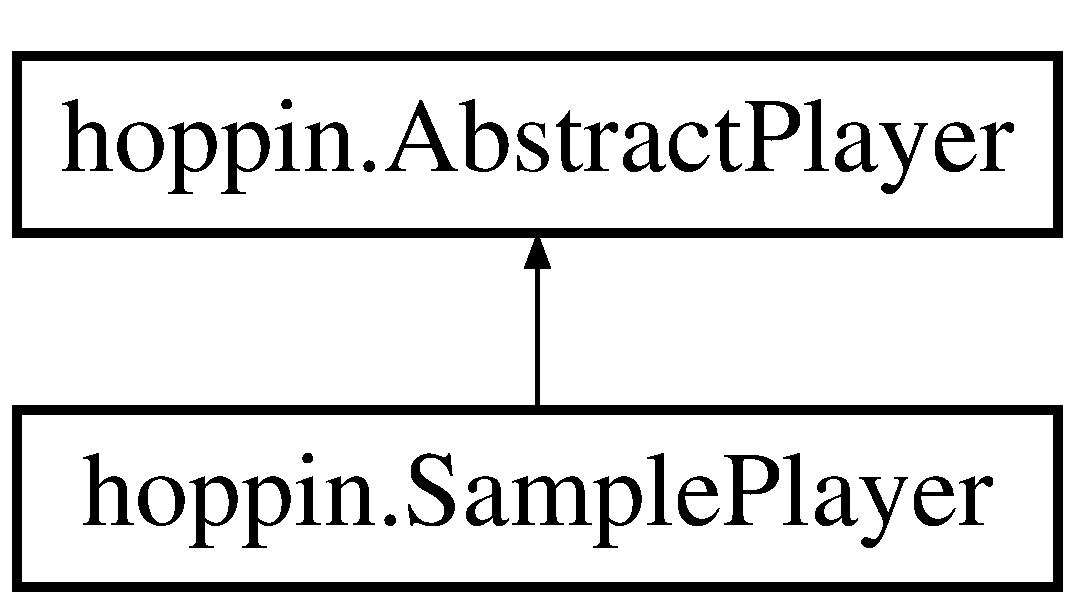
\includegraphics[height=2.000000cm]{da/d2e/classhoppin_1_1_abstract_player}
\end{center}
\end{figure}
\subsection*{公開メンバ関数}
\begin{DoxyCompactItemize}
\item 
abstract Player\+Move \hyperlink{classhoppin_1_1_abstract_player_a0f8f66f25014638ed78e82b294b4b306}{move} ()
\end{DoxyCompactItemize}


\subsection{詳解}


 Abstract\+Player.\+cs の 9 行目に定義があります。



\subsection{メソッド詳解}
\index{hoppin\+::\+Abstract\+Player@{hoppin\+::\+Abstract\+Player}!move@{move}}
\index{move@{move}!hoppin\+::\+Abstract\+Player@{hoppin\+::\+Abstract\+Player}}
\subsubsection[{\texorpdfstring{move()}{move()}}]{\setlength{\rightskip}{0pt plus 5cm}abstract Player\+Move hoppin.\+Abstract\+Player.\+move (
\begin{DoxyParamCaption}
{}
\end{DoxyParamCaption}
)\hspace{0.3cm}{\ttfamily [pure virtual]}}\hypertarget{classhoppin_1_1_abstract_player_a0f8f66f25014638ed78e82b294b4b306}{}\label{classhoppin_1_1_abstract_player_a0f8f66f25014638ed78e82b294b4b306}


このクラス詳解は次のファイルから抽出されました\+:\begin{DoxyCompactItemize}
\item 
Game\+System/\hyperlink{_abstract_player_8cs}{Abstract\+Player.\+cs}\end{DoxyCompactItemize}

\hypertarget{classhoppin_1_1_hoppin_u_i}{}\section{hoppin.\+Hoppin\+UI Class Reference}
\label{classhoppin_1_1_hoppin_u_i}\index{hoppin.\+Hoppin\+UI@{hoppin.\+Hoppin\+UI}}
Inheritance diagram for hoppin.\+Hoppin\+UI\+:\begin{figure}[H]
\begin{center}
\leavevmode
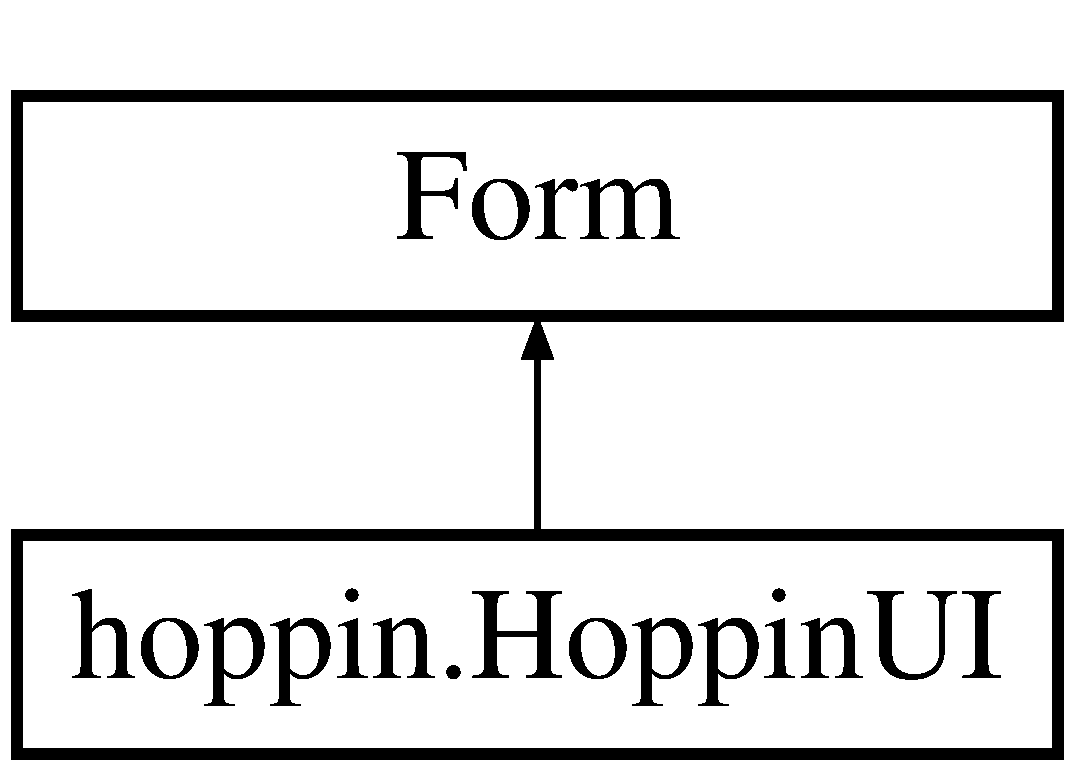
\includegraphics[height=2.000000cm]{classhoppin_1_1_hoppin_u_i}
\end{center}
\end{figure}
\subsection*{Public Member Functions}
\begin{DoxyCompactItemize}
\item 
{\bfseries Hoppin\+UI} (\hyperlink{classhoppin_1_1_game_system_1_1_game_manager}{Game\+Manager} game\+Manager)\hypertarget{classhoppin_1_1_hoppin_u_i_a7faed3d0cc7a679dad7800bd1ab6d4a9}{}\label{classhoppin_1_1_hoppin_u_i_a7faed3d0cc7a679dad7800bd1ab6d4a9}

\end{DoxyCompactItemize}
\subsection*{Protected Member Functions}
\begin{DoxyCompactItemize}
\item 
override void \hyperlink{classhoppin_1_1_hoppin_u_i_a4ebb6fb66a82f87ac8c53665958ba151}{On\+Paint} (Paint\+Event\+Args e)
\begin{DoxyCompactList}\small\item\em 描画インタフェース \end{DoxyCompactList}\item 
override void \hyperlink{classhoppin_1_1_hoppin_u_i_a6bb97d2a8631997b34eb333080958c23}{Dispose} (bool disposing)
\begin{DoxyCompactList}\small\item\em 使用中のリソースをすべてクリーンアップします。 \end{DoxyCompactList}\end{DoxyCompactItemize}


\subsection{Member Function Documentation}
\index{hoppin\+::\+Hoppin\+UI@{hoppin\+::\+Hoppin\+UI}!Dispose@{Dispose}}
\index{Dispose@{Dispose}!hoppin\+::\+Hoppin\+UI@{hoppin\+::\+Hoppin\+UI}}
\subsubsection[{\texorpdfstring{Dispose(bool disposing)}{Dispose(bool disposing)}}]{\setlength{\rightskip}{0pt plus 5cm}override void hoppin.\+Hoppin\+U\+I.\+Dispose (
\begin{DoxyParamCaption}
\item[{bool}]{disposing}
\end{DoxyParamCaption}
)\hspace{0.3cm}{\ttfamily [protected]}}\hypertarget{classhoppin_1_1_hoppin_u_i_a6bb97d2a8631997b34eb333080958c23}{}\label{classhoppin_1_1_hoppin_u_i_a6bb97d2a8631997b34eb333080958c23}


使用中のリソースをすべてクリーンアップします。 


\begin{DoxyParams}{Parameters}
{\em disposing} & マネージ リソースが破棄される場合 true、破棄されない場合は false です。\\
\hline
\end{DoxyParams}
\index{hoppin\+::\+Hoppin\+UI@{hoppin\+::\+Hoppin\+UI}!On\+Paint@{On\+Paint}}
\index{On\+Paint@{On\+Paint}!hoppin\+::\+Hoppin\+UI@{hoppin\+::\+Hoppin\+UI}}
\subsubsection[{\texorpdfstring{On\+Paint(\+Paint\+Event\+Args e)}{OnPaint(PaintEventArgs e)}}]{\setlength{\rightskip}{0pt plus 5cm}override void hoppin.\+Hoppin\+U\+I.\+On\+Paint (
\begin{DoxyParamCaption}
\item[{Paint\+Event\+Args}]{e}
\end{DoxyParamCaption}
)\hspace{0.3cm}{\ttfamily [protected]}}\hypertarget{classhoppin_1_1_hoppin_u_i_a4ebb6fb66a82f87ac8c53665958ba151}{}\label{classhoppin_1_1_hoppin_u_i_a4ebb6fb66a82f87ac8c53665958ba151}


描画インタフェース 


\begin{DoxyParams}{Parameters}
{\em e} & \\
\hline
\end{DoxyParams}


The documentation for this class was generated from the following files\+:\begin{DoxyCompactItemize}
\item 
Game\+System/Hoppin\+U\+I.\+cs\item 
Game\+System/Hoppin\+U\+I.\+Designer.\+cs\end{DoxyCompactItemize}

\hypertarget{classhoppin_1_1_sample_player}{}\section{hoppin.\+Sample\+Player Class Reference}
\label{classhoppin_1_1_sample_player}\index{hoppin.\+Sample\+Player@{hoppin.\+Sample\+Player}}
Inheritance diagram for hoppin.\+Sample\+Player\+:\begin{figure}[H]
\begin{center}
\leavevmode
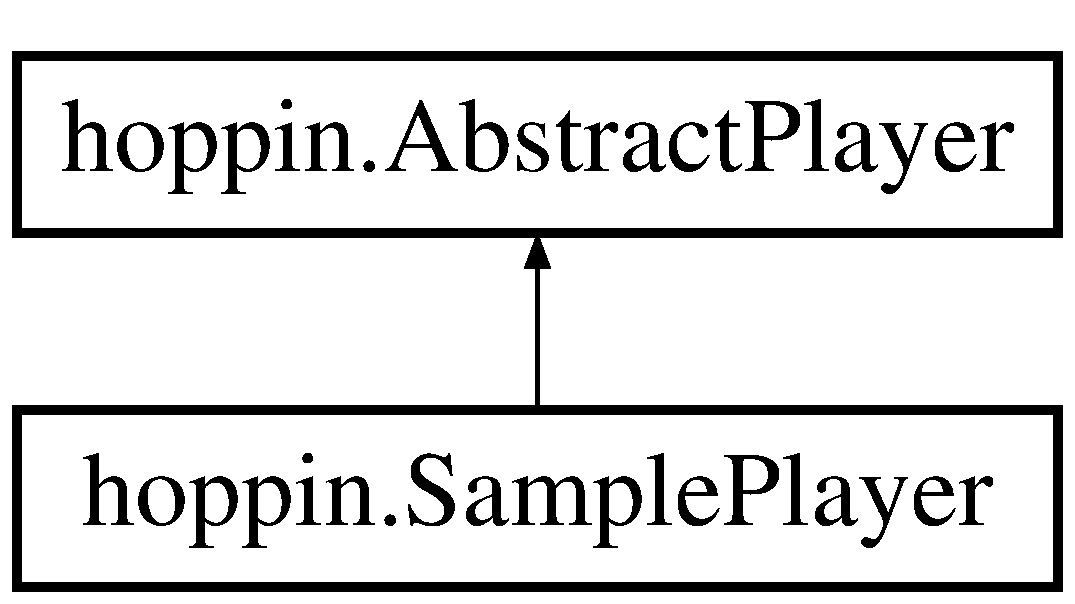
\includegraphics[height=2.000000cm]{classhoppin_1_1_sample_player}
\end{center}
\end{figure}
\subsection*{Public Member Functions}
\begin{DoxyCompactItemize}
\item 
{\bfseries Sample\+Player} (string name)\hypertarget{classhoppin_1_1_sample_player_ab54d749ed27ffe85c01f939cdb4c5c70}{}\label{classhoppin_1_1_sample_player_ab54d749ed27ffe85c01f939cdb4c5c70}

\item 
override Player\+Move {\bfseries move} ()\hypertarget{classhoppin_1_1_sample_player_a6a27c215c5363baf80910f5d44385c7f}{}\label{classhoppin_1_1_sample_player_a6a27c215c5363baf80910f5d44385c7f}

\end{DoxyCompactItemize}
\subsection*{Additional Inherited Members}


The documentation for this class was generated from the following file\+:\begin{DoxyCompactItemize}
\item 
hoppin/\+Sample\+Player/Sample\+Player.\+cs\end{DoxyCompactItemize}

\chapter{ファイル詳解}
\hypertarget{_abstract_player_8cs}{}\section{Game\+System/\+Abstract\+Player.cs File Reference}
\label{_abstract_player_8cs}\index{Game\+System/\+Abstract\+Player.\+cs@{Game\+System/\+Abstract\+Player.\+cs}}
\subsection*{Classes}
\begin{DoxyCompactItemize}
\item 
class \hyperlink{classhoppin_1_1_abstract_player}{hoppin.\+Abstract\+Player}
\begin{DoxyCompactList}\small\item\em 今回作成していただくプレイヤーの抽象クラスです. ゲーム側は\+Get\+Move()を使用してプレイヤーの動作を決定しています. 使用できる関数は参照値を返すため,取得したデータをそのまま変更すると,関数から取得できる値も変更されてしまいます. \end{DoxyCompactList}\end{DoxyCompactItemize}
\subsection*{Namespaces}
\begin{DoxyCompactItemize}
\item 
namespace \hyperlink{namespacehoppin}{hoppin}
\end{DoxyCompactItemize}

\hypertarget{_hoppin_u_i_8cs}{}\section{Game\+System/\+Hoppin\+UI.cs ファイル}
\label{_hoppin_u_i_8cs}\index{Game\+System/\+Hoppin\+U\+I.\+cs@{Game\+System/\+Hoppin\+U\+I.\+cs}}
\subsection*{クラス}
\begin{DoxyCompactItemize}
\item 
class \hyperlink{classhoppin_1_1_hoppin_u_i}{hoppin.\+Hoppin\+UI}
\end{DoxyCompactItemize}
\subsection*{名前空間}
\begin{DoxyCompactItemize}
\item 
namespace \hyperlink{namespacehoppin}{hoppin}
\end{DoxyCompactItemize}

\hypertarget{_hoppin_u_i_8_designer_8cs}{}\section{Game\+System/\+Hoppin\+UI.Designer.\+cs ファイル}
\label{_hoppin_u_i_8_designer_8cs}\index{Game\+System/\+Hoppin\+U\+I.\+Designer.\+cs@{Game\+System/\+Hoppin\+U\+I.\+Designer.\+cs}}
\subsection*{クラス}
\begin{DoxyCompactItemize}
\item 
class \hyperlink{classhoppin_1_1_hoppin_u_i}{hoppin.\+Hoppin\+UI}
\end{DoxyCompactItemize}
\subsection*{名前空間}
\begin{DoxyCompactItemize}
\item 
namespace \hyperlink{namespacehoppin}{hoppin}
\end{DoxyCompactItemize}

\hypertarget{_temporary_generated_file__036_c0_b5_b-1481-4323-8_d20-8_f5_a_d_c_b23_d92_8cs}{}\section{obj/\+Debug/\+Temporary\+Generated\+File\+\_\+036\+C0\+B5\+B-\/1481-\/4323-\/8\+D20-\/8\+F5\+A\+D\+C\+B23\+D92.cs ファイル}
\label{_temporary_generated_file__036_c0_b5_b-1481-4323-8_d20-8_f5_a_d_c_b23_d92_8cs}\index{obj/\+Debug/\+Temporary\+Generated\+File\+\_\+036\+C0\+B5\+B-\/1481-\/4323-\/8\+D20-\/8\+F5\+A\+D\+C\+B23\+D92.\+cs@{obj/\+Debug/\+Temporary\+Generated\+File\+\_\+036\+C0\+B5\+B-\/1481-\/4323-\/8\+D20-\/8\+F5\+A\+D\+C\+B23\+D92.\+cs}}

\hypertarget{_temporary_generated_file__5937a670-0e60-4077-877b-f7221da3dda1_8cs}{}\section{obj/\+Debug/\+Temporary\+Generated\+File\+\_\+5937a670-\/0e60-\/4077-\/877b-\/f7221da3dda1.cs ファイル}
\label{_temporary_generated_file__5937a670-0e60-4077-877b-f7221da3dda1_8cs}\index{obj/\+Debug/\+Temporary\+Generated\+File\+\_\+5937a670-\/0e60-\/4077-\/877b-\/f7221da3dda1.\+cs@{obj/\+Debug/\+Temporary\+Generated\+File\+\_\+5937a670-\/0e60-\/4077-\/877b-\/f7221da3dda1.\+cs}}

\hypertarget{_temporary_generated_file___e7_a71_f73-0_f8_d-4_b9_b-_b56_e-8_e70_b10_b_c5_d3_8cs}{}\section{obj/\+Debug/\+Temporary\+Generated\+File\+\_\+\+E7\+A71\+F73-\/0\+F8\+D-\/4\+B9\+B-\/\+B56\+E-\/8\+E70\+B10\+B\+C5\+D3.cs ファイル}
\label{_temporary_generated_file___e7_a71_f73-0_f8_d-4_b9_b-_b56_e-8_e70_b10_b_c5_d3_8cs}\index{obj/\+Debug/\+Temporary\+Generated\+File\+\_\+\+E7\+A71\+F73-\/0\+F8\+D-\/4\+B9\+B-\/\+B56\+E-\/8\+E70\+B10\+B\+C5\+D3.\+cs@{obj/\+Debug/\+Temporary\+Generated\+File\+\_\+\+E7\+A71\+F73-\/0\+F8\+D-\/4\+B9\+B-\/\+B56\+E-\/8\+E70\+B10\+B\+C5\+D3.\+cs}}

\hypertarget{_program_8cs}{}\section{Program.\+cs ファイル}
\label{_program_8cs}\index{Program.\+cs@{Program.\+cs}}
\subsection*{クラス}
\begin{DoxyCompactItemize}
\item 
class {\bfseries hoppin.\+Program}
\begin{DoxyCompactList}\small\item\em ゲームシステムのクラス \end{DoxyCompactList}\end{DoxyCompactItemize}
\subsection*{名前空間}
\begin{DoxyCompactItemize}
\item 
namespace \hyperlink{namespacehoppin}{hoppin}
\end{DoxyCompactItemize}

\hypertarget{_assembly_info_8cs}{}\section{Properties/\+Assembly\+Info.cs ファイル}
\label{_assembly_info_8cs}\index{Properties/\+Assembly\+Info.\+cs@{Properties/\+Assembly\+Info.\+cs}}

\hypertarget{_resources_8_designer_8cs}{}\section{Properties/\+Resources.Designer.\+cs ファイル}
\label{_resources_8_designer_8cs}\index{Properties/\+Resources.\+Designer.\+cs@{Properties/\+Resources.\+Designer.\+cs}}
\subsection*{クラス}
\begin{DoxyCompactItemize}
\item 
class {\bfseries hoppin.\+Properties.\+Resources}
\begin{DoxyCompactList}\small\item\em ローカライズされた文字列などを検索するための、厳密に型指定されたリソース クラスです。 \end{DoxyCompactList}\end{DoxyCompactItemize}
\subsection*{名前空間}
\begin{DoxyCompactItemize}
\item 
namespace \hyperlink{namespacehoppin_1_1_properties}{hoppin.\+Properties}
\end{DoxyCompactItemize}

\hypertarget{_settings_8_designer_8cs}{}\section{Properties/\+Settings.Designer.\+cs ファイル}
\label{_settings_8_designer_8cs}\index{Properties/\+Settings.\+Designer.\+cs@{Properties/\+Settings.\+Designer.\+cs}}
\subsection*{クラス}
\begin{DoxyCompactItemize}
\item 
class {\bfseries hoppin.\+Properties.\+Settings}
\end{DoxyCompactItemize}
\subsection*{名前空間}
\begin{DoxyCompactItemize}
\item 
namespace \hyperlink{namespacehoppin_1_1_properties}{hoppin.\+Properties}
\end{DoxyCompactItemize}

\hypertarget{_sample_player_8cs}{}\section{Sample\+Player/\+Sample\+Player.cs ファイル}
\label{_sample_player_8cs}\index{Sample\+Player/\+Sample\+Player.\+cs@{Sample\+Player/\+Sample\+Player.\+cs}}
\subsection*{クラス}
\begin{DoxyCompactItemize}
\item 
class \hyperlink{classhoppin_1_1_sample_player}{hoppin.\+Sample\+Player}
\end{DoxyCompactItemize}
\subsection*{名前空間}
\begin{DoxyCompactItemize}
\item 
namespace \hyperlink{namespacehoppin}{hoppin}
\end{DoxyCompactItemize}

%--- End generated contents ---

% Index
\backmatter
\newpage
\phantomsection
\clearemptydoublepage
\addcontentsline{toc}{chapter}{索引}
\printindex

\end{document}
